% 2.1.Download.tex
%	Last update: 2019/07/22 F.Kanehori
%newpage
\subsection{Springheadライブラリのダウンロード}
\label{subsec:Download}

\noindent
まずSpringhead LibraryをGitHubからダウンロード(clone)してください。
以下、ダウンロードするディレクトリを\SprTop{}として説明を進めます。

\medskip
\begin{narrow}[15pt]
	\CmndBox{%
		> chdir C:/Springhead\\
		> git clone --recurse-submodules\Cont\\
		\Hskip{100pt}https://github.com/sprphys/Springhead
	}
\end{narrow}
\medskip
サブモジュールを選択する場合は
\begin{narrow}[15pt]
	\CmndBox{%
		> chdir C:/Springhead\\
		> git clone https://github.com/sprphys/Springhead\\
		> git submodule update --init --checkout buildtool\\
		> git submodule update --init --checkout dependency
	}
\end{narrow}
\medskip
GUIの場合は
\begin{narrow}[15pt]
	\begin{figure}[h]
	\begin{center}
	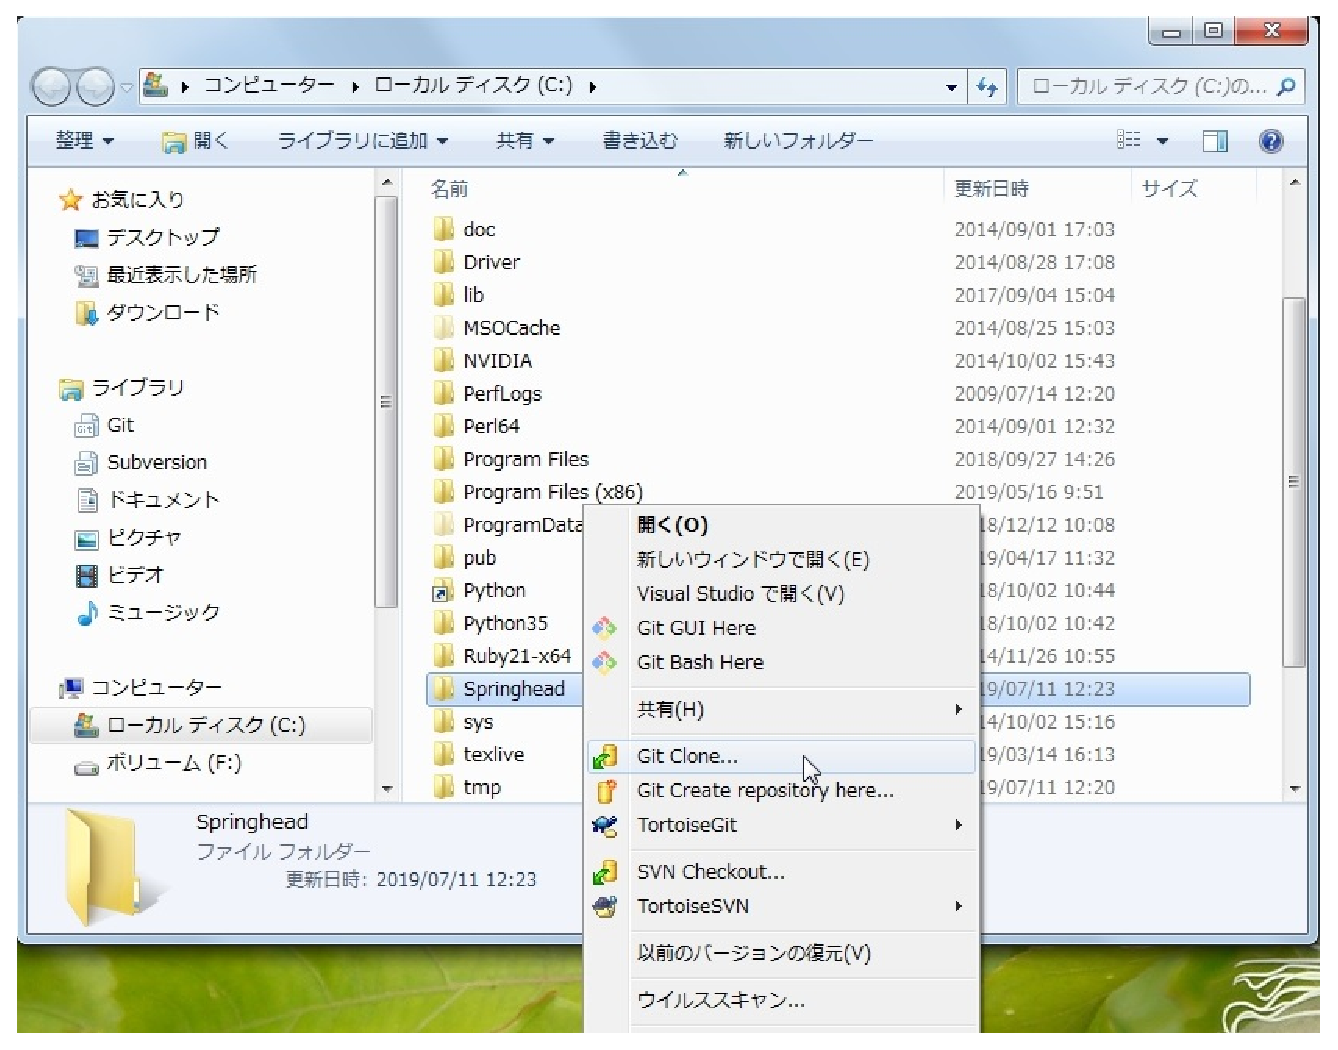
\includegraphics[width=0.5\textwidth]{fig/SpringheadClone1.eps}
	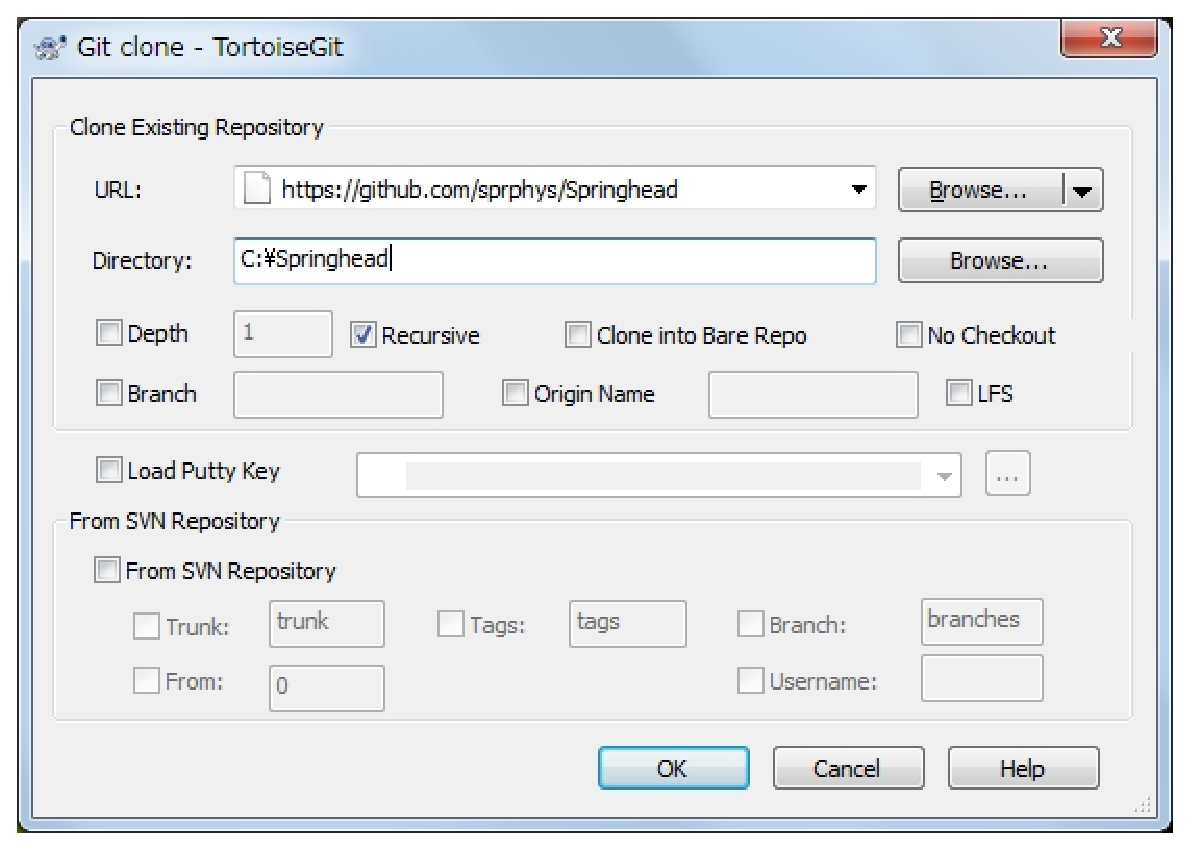
\includegraphics[width=0.4\textwidth]{fig/SpringheadClone2.eps}
	\end{center}
	\caption{Springheadダウンロード}
	\label{fig:SpringheadClone}
	\end{figure}
\end{narrow}

% end: 2.1.Download.tex
